\section{Concepts and Definitions}\label{sec:concepts}
%
All concepts, definitions, and algorithms discussed in this article
are illustrated on a commonly used dynamic system consisting of water
tanks that are connected with valves.
%
\subsection{Running Example}
%
The three-tank system is shown in figure~\ref{fig:three_tanks}. The
tanks are denoted as $T_1$, $T_2$, and $T_3$. They all have the
same area $A_1 = A_2 = A_3 = 3~[\textrm{m}^2]$. The three tanks are
indestructible and of infinite height, so no overfills or anything
like that happens (the experiment is idealized). The experiments is
performed on a planet similar to ours where $g = 10$ and the liquid is
``pure'' water with density $\rho = 1$.
%
\begin{figure}[htb]
  \centering
  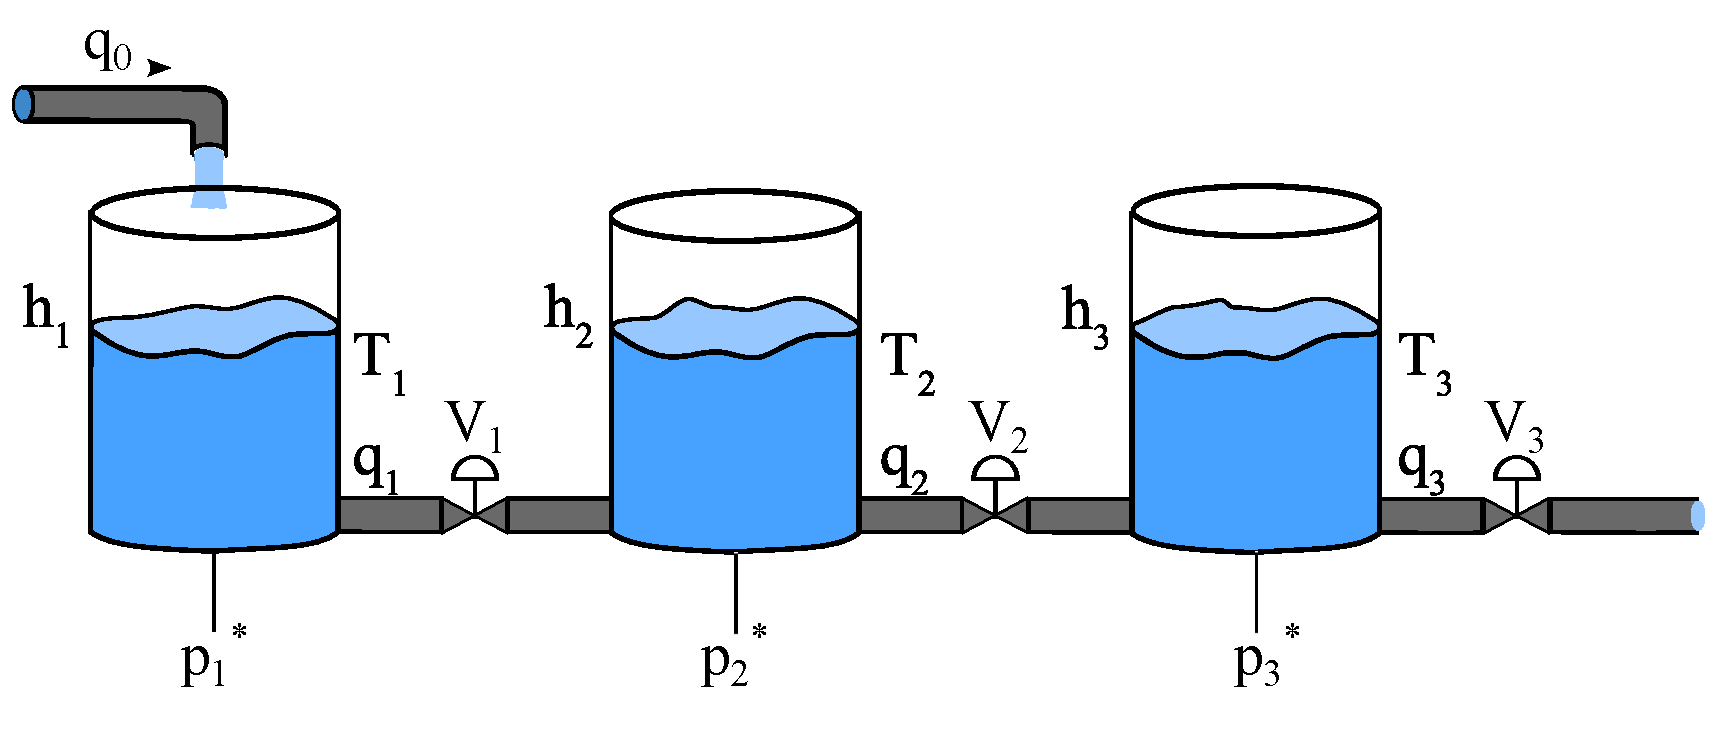
\includegraphics[width=1\columnwidth]{3-tanks}
  \caption{Diagram of the three-tank system.}
  \label{fig:three_tanks}
\end{figure}
\par\noindent
%
Tank $T_1$ gets filled from a pipe $q_0$ with a constant flow of
$0.75~[\textrm{m}^3/\textrm{s}]$. It drains into $T_2$ via a pipe
$q_1$. The liquid level is denoted as $h_1$. There is a pressure
sensor $p_1$ connected to $T_1$ that measures the pressure in Pascals
[Pa]. Starting from the Newton's (and Bernouli's) equations and
manipulating them (the actual derivation is trivial and irrelevant in
this paper) we derive the following Ordinary Differential Equation
(ODE) that gives the level of the liquid in $T_1$:
%
\begin{eqnarray}
%
\frac{d h_1}{dt} = \frac{q_0 - k_1 \sqrt{h_1}}{A_1}\label{eq:ode1}
%
\end{eqnarray}
%
In eq.~\ref{eq:ode1}, the coefficient $k_1$ is the product of the
cross-sectional area of the tank $A_1$ and the area of the drainage
hole and $\sqrt{2g}$ and the friction/contraction factor of the
hole. We emphasize the use of $k_1$ because, later, we will be
``diagnosing'' our system in term of changes in $k_1$. Consider a
physical valve $R_1$ between $T_1$ and $T_2$ that constraints the flow
between the two tanks. We can say that the valve changes
proportionally the cross-sectional drainage area of $q_1$ and hence
$k_1$. The diagnostic task will be to compute the true value of $k_1$,
given $p_1$, and from $k_1$ we can compute the actual position of the
valve $R_1$.
%
The water levels of $T_2$ and $T_3$, denoted as $h_2$ and $h_3$
respectively, are given by:
%
\begin{eqnarray}\label{eq:tank1}
%
\frac{d h_i}{dt} = \frac{k_{i - 1} \sqrt{h_{i - 1}} - k_i \sqrt{h_i}}{A_i},
%
\end{eqnarray}
%
where $i$ is the tank index ($i \in \{2, 3\}$).
\par
Let us say that $k_1 = 0.25$, $k_2 = 0.5$, and $k_3 = 0.75$ (these
values have no physical meaning, we have chosen them to produce
``nice'' simulation results).
\par
Finally, we turn the water level into pressure:
\begin{eqnarray}
p_i = \frac{g\,h_i\,A}{A} = g\,h_i
\end{eqnarray}
where $i$ is the tank index ($i \in \{1, 2, 3\}$).
\par
It is assumed that the initial water level in the three tanks is zero.
%
Let us continue with some notation and definitions.
%
\subsection{Simulation Model Classes}
%
We assume a (simulation) model to consist of a set of equations $\Phi$
describing the behavior of a system \sd.

In this article we examine several different types of model for
simulation, including dynamical, linear, and qualitative. For our
models, we consider three classes of variables: $\vec{x}(t)$ is the
state variable vector, $\vec{u}(t)$ is the input variable vector, and
$\vec{y}(t)$ is the observation vector. In addition to that,
$\vec{\omega}(t)$ is a disturbance vector.

\begin{definition}[Non-Linear Dynamical Model $\Phi_D$]
We write the dynamical equations for a model in state-space form using
\begin{eqnarray}\label{dyn-model}
%\frac{d \vec{x}(t)}{dt} & = & \psi (\vec{x}(t)) + \vec{u}(t))\\
\dot{\vec{x}}(t) & = & \psi (\vec{x}(t)) + \vec{u}(t))\\
\vec{y}(t) & = & \gamma (\vec{x}(t)), \vec{u}(t)),
\end{eqnarray}
where $\psi$ and $\gamma$ are non-linear functions.
\end{definition}

\begin{definition}[Linear Dynamical Model $\Phi_L$]
We write the linear dynamical equations for a model in state-space form using
\begin{eqnarray}\label{linear-model}
\dot{\vec{x}}(t) & = & \mathbf{A} \vec{x}(t) + \mathbf{B} \vec{u}(t)) + \mathbf{C} \vec{\omega}(t) +  \vec{\omega}(t)\\
\vec{y}(t) & = & \mathbf{D} (\vec{x}(t)),
\end{eqnarray}
where $\mathbf{A}, ~ \mathbf{B},~\mathbf{C}$ and $\mathbf{D}$ are linear matrices.
%---------------
\end{definition}

\begin{definition}[Qualitative Model $\Phi_Q$]
We write the dynamical equations for a model in state-space form using
\begin{eqnarray}\label{qual-model}
\dot{\vec{x}}(t) & = & \upsilon (\vec{x}(t)) + \vec{u}(t))\\
\vec{y}(t) & = & \mu (\vec{x}(t)), \vec{u}(t)),
\end{eqnarray}
where $\upsilon$ and $\mu$ are  functions from the set of reasonable functions $f$ such that $f' > 0$ on the interior of its domain \citep{kuipers1994composition}.
%---------------
\end{definition}

\begin{definition}[Boolean Model $\Phi_B$]
We write the dynamical equations for a model in state-space form using
\begin{eqnarray}\label{boolean-model}
\frac{d \vec{x}(t)}{dt} & = & \upsilon (\vec{x}(t)) + \vec{u}(t))\\
\vec{y}(t) & = & \mu (\vec{x}(t)), \vec{u}(t)),
\end{eqnarray}
where $\upsilon$ and $\mu$ are  functions from the set of reasonable functions $f$ such that $f' > 0$ on the interior of its domain \citep{kuipers1994composition}.
%---------------
\end{definition}

\subsection{Compositional Modeling}
%
We are interested in system models that are explicitly decomposable,
so we must capture not just the behavioral equations, but also a
framework that captures the system's compositional properties.


A domain $D$ is \textit{compositional} if a system model from $D$ can
be composed from model components, each of which is defined by a
component behavioral model.

A system is compositional if its behavior consists of the combination
of the behaviors of its constituent components' behaviors. A
precondition for compositional modelling is the existence of an
underlying structure for the model.  We can thus describe a
decomposable model $\Psi$ using two orthogonal aspects: {\em behavior}
and {\em topology (interaction)}. The behavior model describes the
(possibly dynamic) behaviors of the system and components; the
topology model describes the component connectivity in terms of
components and their connections, and defines the constraints on
component behaviors that enable their interactions to specify the
system-level interaction \cite{GosslerS05}.

The topology of a system describes how the components are connected.

\begin{definition}
%
We describe system topology of a composable system $\Psi$ using a
graph $G(V,E)$, where vertices $V$ correspond to components and edges
in $E$ correspond to connections between components.
%
\end{definition}

\begin{definition}
%
A composable system $\Psi$ is defined using the pair $(G,{\Phi})$,
where $G$ is the topology model and ${\Phi}$ is the behavior model.
%
\end{definition}

We assume that a system $\Psi$ can be decomposed into sub-systems.
There are two types of sub-system: a component, which is a primitive
sub-system, and a composite sub-system, which can be further
decomposed. A component represents the specification of a primitive
behavioral specification of $\Psi$, i.e, no further decomposition of
behavior is possible that allows each sub-function to coherently
describe a process. We assume a set ${\cal C}=\{C_1,...,C_m\}$ of
components, and that the input/output tuple for each $C_j$ can be
specified.

% using the tuple $(\mbox{\boldmath$U$}_j(t),\mbox{\boldmath$Y$}_j(t))$.

By merging components and/or sub-systems, we can define a hierarchical
model; we define a flat model to consist of a system represented only
in terms of components $C_i \in {\cal C}$ and their interconnections.

To generate models, we use a collection of pre-defined component models, called a 
component library.

%-- component library (multiple component types per component)
%-- topology --- an interconnection graph (or tree if you like)
%-- system description (model)
%-- observation - variable assignment (obs) + time


%----------------------------------
\subsection{Diagnosis Model}
%----------------------------------

A simulation model identifies only a single set of \textit{ideal}
conditions under which the model applies. More generally, real-world
systems require models that can simulate over multiple possible modes,
where a mode is a set of conditions under which the system is
operating. For example, a car can drive in a range of gears (forward
and reverse), and the dynamics of each gear are different and require
different simulation models. In addition to these nominal modes, we
can identify a set of failure modes, where the system is operating
given some level of degradation.  We distinguish two classes of mode,
nominal modes ${\Omega}_N$ and failure modes ${\Omega}_F$.


We now introduce a \textit{diagnosis model}.  
 

\begin{definition}[Diagnosis Model]
A diagnosis model for system $S$ consists of a set of mode-specific
equations, i.e., equation set $\Phi_i$ is associated with a mode
$\omega_i$, using the pair $(\omega,{\Phi}_{\omega})$.
\end{definition}

The generalized notion of model now becomes $({\Omega},{\Phi})$, where
the equations can be dynamical, linear, qualitative or Boolean.

In terms of component models, each component $C_i$ has associated
mode-variable $\omega_i$; $\omega_i$ can be functioning normally
($[\omega_i = OK]$), or can take on a finite set of abnormal
behaviors.

\subsection{Diagnostic Problem}
%
\begin{definition}[Observation]
%
Given a system description \sd, an observation $\tilde\alpha =
\langle\alpha, t_{\mathrm{obs}}\rangle$ is an instantiation of the
variables in \obs at a time instant $t_{\mathrm{obs}}$.
%
\end{definition}
%
\begin{definition}[Fault Injection]
%
Given a system description \sd, a fault injection $\tilde{\varepsilon}
= \langle\varepsilon, t_{\mathrm{inj}}\rangle$ is an instantiation of
the variables in \comps at a time instant $t_{\mathrm{inj}}$.
%
\end{definition}
%
\begin{definition}[Diagnosis]
%
Given a system description \sd, a diagnosis $\tilde{\omega} =
\langle\omega, t_{\mathrm{diag}}\rangle$ is a probabilistic assignment
of the variables in \comps at a time instant $t_{\mathrm{diag}}$.
%
\end{definition}
%
\begin{definition}[Diagnostic Problem]
%
A diagnostic problem \dproblem is defined as the quadruple $\dproblem
= \langle\sd, \tilde{\alpha}, \tilde{\varepsilon},
\tilde{\omega}\rangle$.
%
\end{definition}
%
\subsection{Diagnostic Performance Metrics}
%
Unlike other AI disciplines such as satisfiability where algorithm
performance is typically measured by computational efficiency, in MBD
there are multiple factor that should be considered when applying to
real-world systems. The most important computational metric is the
number of diagnostic errors which is dual to the isolation accuracy
\cite{feldman10empirical}.
%
\begin{definition}[Diagnostic Errors]
%
Given a diagnostic problem \dproblem the diagnostic errors metric
$M_{\mathrm{err}}$ is defined as:
%
\begin{eqnarray}
%
M_{\mathrm{err}} = \sum_{c \in \comps}{\left|\pr(\omega_c \ne \ok) - \inj(\varepsilon_c)\right|}
%
\end{eqnarray}
%
\end{definition}
%
The second most important metric for dynamic system is the time
between the fault injection and the algorithm ``thinks'' there is a
fault.
%
\begin{definition}[Isolation Time]
%
Given a diagnostic problem \dproblem the isolation time metric
$M_{\mathrm{iso}}$ is defined as:
%
\begin{eqnarray}
%
M_{\mathrm{iso}} = t_{\mathrm{diag}} - t_{\mathrm{inj}}
%
\end{eqnarray}
%
\end{definition}
%
Diagnostic algorithms are typically given a system model \sd and a set
of test cases $\mathcal{A} = \left\{\langle\tilde\alpha_1,
\tilde\varepsilon_1\rangle, \langle\tilde\alpha_2,
\tilde\varepsilon_2\rangle, \cdots, \langle\tilde\alpha_n,
\tilde\varepsilon_n\rangle\right\}$. The main goal of these diagnostic
algorithm is to optimize a superposition of the diagnostic
metrics. Each diagnostic metric is weighted with a domain specific
coefficient (these are $g_{\mathrm{err}}$, and $g_{\mathrm{iso}}$,
respectively, in the the cases of $M_{\mathrm{err}}$, and
$M_{\mathrm{iso}}$). In this article, however, we solve an orthogonal
problem: given a diagnostic algorithm, a component library and a set
of test cases $\mathcal{A}$, compute a model composition \sd such that
$g_{\mathrm{err}}M_{\mathrm{err}} + g_{\mathrm{iso}}M_{\mathrm{iso}}$
is minimized.
